\documentclass{article}

\usepackage[utf8]{inputenc}
\usepackage{graphicx}

\usepackage{hyperref}
\renewcommand*{\figureautorefname}{Figura}

\usepackage{caption}
\usepackage{float}
\usepackage{epigraph}
\usepackage{multicol}
\usepackage[bottom,flushmargin]{footmisc}

\usepackage{adjustbox}
\usepackage{tikz}
\usetikzlibrary{
  babel,
  decorations.text,
  decorations.pathreplacing,
  decorations.pathmorphing,
  calc,
  chains,
  automata,
  positioning,
  arrows
}
\tikzset{%
  node distance=3cm, % specifies the minimum distance between two nodes. Change if necessary.
  every state/.style={thick}, % sets the properties for each ’state’ node
  double distance=2.5pt,
  shorten >= 2pt, shorten <= 2pt,
  initial text=\( \),
  every edge/.style={%
    draw,->, >=stealth, auto, semithick
  }
}

\newcommand{\emptystr}{\varepsilon}
\usepackage{hyperref}
\hypersetup{pdfauthor={Cristian Adrián Ontivero}}
\usetikzlibrary{shapes}
\graphicspath{{imgs/}}

\newlength\tindent
\setlength{\tindent}{\parindent}
\setlength{\parindent}{0pt}
\renewcommand{\indent}{\hspace*{\tindent}}

%These tell TeX which packages to use.
\usepackage{array,epsfig}
\usepackage{amsmath}
\usepackage{amsfonts}
\usepackage{amssymb}
\usepackage{amsxtra}
\usepackage{amsthm}
\usepackage{mathrsfs}

%Here I define some theorem styles and shortcut commands for symbols I use often
\theoremstyle{definition}
\newtheorem{defn}{Definición}
\newtheorem{thm}{Teorema}
\newtheorem{cor}{Corolario}
\newtheorem*{rmk}{Remark}
\newtheorem{lem}{Lema}
\newtheorem*{joke}{Joke}

\newtheorem{ex}{Ejemplo}
\newcommand{\exautorefname}{Ejemplo}

\newtheorem{exercise}{Ejercicio}
\newcommand{\exerciseautorefname}{Ejercicio}

\newtheorem{soln}{Solución}
\newtheorem{prop}{Proposición}

%Pagination stuff.
\setlength{\topmargin}{-.3 in}
\setlength{\oddsidemargin}{0in}
\setlength{\evensidemargin}{0in}
\setlength{\textheight}{9.in}
\setlength{\textwidth}{6.5in}
\pagestyle{empty}

\def\isodate{\leavevmode\hbox{\the\year-\twodigits\month-\twodigits\day}}
\def\twodigits#1{\ifnum#1<10 0\fi\the#1}
\begin{document}
\begin{center}
  {\LARGE Notas Sobre Máquinas de Turing}\\[.2cm]
  Cristian Adrián Ontivero \\[.05cm]%
  \isodate
\end{center}

Para hacer una máquina que acepte cadenas binarias con paridad par (o peso de
Hamming par), basta con un DFA, pero en el siguiente ejemplo lo haremos con
una máquina de Turing.

Es decir, la idea es construir una máquina de Turing que acepte una cadena
binaria si la cantidad de {\tt 1}s es par, y de lo contrario, la rechace. Por
ejemplo, dada la siguiente cinta con el cabezal apuntando al comienzo de la
cadena de entrada:

\begin{center}
 \begin{tikzpicture}
  \tikzset{tape/.style={minimum size=.5cm, draw, font=\tt}}
\begin{scope}[start chain=0 going right, node distance=0mm]
  \foreach \x [count=\i] in {0,1,1,0,\textvisiblespace,\textvisiblespace}{%
    \ifnum\i=6 % if last node reset outer sep to 0pt
      \node [on chain=0, tape, outer sep=0pt] (n\i) {\x};
      \draw (n\i.north east) -- ++(.1,0) decorate [decoration={zigzag,
      segment length=.12cm, amplitude=.02cm}] {-- ($(n\i.south east)+(+.1,0)$)} -- (n\i.south east) -- cycle;
     \else
        \ifnum\i=1
        \node [on chain=0, tape, outer sep=0pt] (n\i) {\x};
        \draw (n\i.north west) -- ++(-.1,0) decorate [decoration={zigzag,
        segment length=.12cm, amplitude=.2mm}] {-- ($(n\i.south west)+(-.1,0)$)}
        -- (n\i.south west) -- cycle;
        \else
          \node [on chain=0, tape] (n\i) {\x};
        \fi
     \fi
   }
   %\node [right=.25cm of n11] {\(\cdots\)};
   \node [tape, below=5mm of n1] (q0) {\(q_0\)};
   \draw [>=latex, ->] (q0) to (n1);
  \end{scope}
 \end{tikzpicture}
\end{center}
Una solución simple sería recorrer la cinta partiendo de un estado inicial
\(q_0\), y cambiar de estado al ver un \(1\), digamos a un estado \(q_1\). De
esta forma, \(q_0\) indica paridad par, mientras que \(q_1\) indica paridad
impar. Si al finalizar la cadena la máquina está en el estado \(q_0\),
acepta. Dado que la definición de máquina de Turing vista en la cátedra
requiere explícitamente de un estado de aceptación, agregamos un estado
\(q_{\text{a}}\) en el que la máquina entra si la cadena se acepta. Razonando
con el ejemplo, llegamos a la siguiente función de transición:
 \begin{align*}
   \delta(q_0, 0) &= (q_0, X, R) \\
   \delta(q_0, 1) &= (q_1, X, R) \\
   \delta(q_1, 0) &= (q_1, X, R) \\
   \delta(q_1, 1) &= (q_1, X, R) \\
   \delta(q_0, \text{\textvisiblespace}) &= (q_{\text{a}}, X, R)
 \end{align*}

El diagrama de estados de la máquina en cuestión se observa en la
\autoref{fig:state_diagram}.

\begin{figure}[ht] % ’ht’ tells LaTeX to place the figure ’here’ or at the top of the page
\centering % centers the figure
\begin{tikzpicture}[node distance=3cm, every edge/.style={draw,->, >=stealth, auto, semithick }]
    \node[state, initial] (q0) {\(q_0\)};
    \node[state, right of=q0] (q1) {\(q_1\)};
    \node[state, accepting, below=1cm of q1] (qa) {\(q_{\text{a}}\)};
    \draw (q0) edge[bend left] node {1/X,R} (q1);
    \draw (q1) edge[bend left] node {1/X,R} (q0);
    \draw (qa) edge[out=180, in=270, <-] node {\textvisiblespace/X,R} (q0);
    \draw (q0) edge[loop above] node {0/X,R} (q0);
    \draw (q1) edge[loop above] node {0/X,R} (q1);
  \end{tikzpicture}
\caption{Diagrama de estados.}\label{fig:state_diagram}
\end{figure}

Para computar, una máquina de Turing se vale de cambios en su estado, en la
cinta, y en dónde apunta la cabecera. Se llama \textbf{configuración} de la
máquina de Turing a una terna de estas cosas. Dadas las cadenas \(\alpha\) y
\(\beta\) sobre el alfabeto de la cinta \(\Gamma\), escribimos \(\alpha~q~\beta\) para
la configuración cuyo estado es \(q\), los contenidos de la cinta son
\(\alpha\beta\), y la cabecera apunta al primer símbolo de \(\beta\). A la derecha
de \(\beta\), la cinta esta vacía (consta sólo de \textvisiblespace). Siguiendo el
ejemplo, la máquina de Turing pasa por las siguientes configuraciones:
\begin{center}
{%
\setlength\tabcolsep{0mm}
\tt
 \begin{tabular}{cccccc}
   \(q_0\) & 0   & 1 & 1 & 0 & \textvisiblespace \\
   X   & \(q_0\) & 1 & 1 & 0 & \textvisiblespace \\
   X   & X & \(q_1\) & 1 & 0 & \textvisiblespace \\
   X   & X & X & \(q_0\) & 0 & \textvisiblespace \\
   X   & X & X & X & \(q_0\) & \textvisiblespace \\
   X   & X & X & X & X & \(q_{\text{a}}\)\\
 \end{tabular}
 }
 \end{center}

Formalmente, definimos la máquina de Turing del ejemplo como una 7-tupla
\((Q, \Sigma, \Gamma, \textvisiblespace, q_0, \delta, F)\) donde:
 \begin{itemize}
   \item \(Q = \{q_0, q_1, q_{\text{a}}\}\)
   \item \(\Sigma = \{{\tt 0,1}\}\)
   \item \(\Gamma = \{{\tt 0,1, X, \textvisiblespace}\}\)
   \item \(\textvisiblespace \in \Gamma \setminus \Sigma\) representa al
   espacio en blanco de la cinta
   \item \(q_0\) es el estado inicial
   \item \(\delta\) es la función de transición (previamente definida)
   \item \(F = \{ q_{\text{a}} \}\)
 \end{itemize}


%\newpage
%\bibliography{refs}
%\bibliographystyle{alpha}

\end{document}


